\documentclass[12pt,a4paper]{article}

\usepackage[T2A]{fontenc} %поддержка кириллицы
\usepackage[utf8]{inputenc} %кодировка текста: koi8-r или utf8 в UNIX, cp1251 в Windows
\usepackage[english,russian]{babel} 
\usepackage[left=2cm,right=1.5cm,top=2cm,bottom=2cm]{geometry} 
\usepackage{tabularx} 
\usepackage{graphicx} 
\usepackage{amsmath} %отображение математической нотации
\usepackage{float}
\usepackage{caption, subcaption} %подписи
%\usepackage{array}
%\usepackage{amsmath,booktabs}
%\usepackage{tabu}
\usepackage{indentfirst}%отступ вначале параграфа
%\usepackage{pscyr} %???
%\usepackage{natbib}
%\usepackage{ragged2e} %для таблиц
 
\captionsetup[table]{labelsep = endash, singlelinecheck=false}
\captionsetup[figure]{name = Рисунок, labelformat=simple, labelsep = endash}

\begin{document}

\newcommand\tline[2]{$\underset{\text{#1}}{\text{\underline{\hspace{#2}}}}$}
\newcommand\nameLine[3]{$\underset{\text{#1}}{\text{\underline{\text{#2}\hspace{#3}}}}$}

\begin{titlepage}
		\centering
		{\fontsize{12pt}{5cm}\selectfont \bfseries Министерство образования и науки Российской Федерации} \\ \vspace{0.5cm}
		{\fontsize{7pt}{5cm}\selectfont ФЕДЕРАЛЬНОЕ ГОСУДАРСТВЕННОЕ АВТОНОМНОЕ ОБРАЗОВАТЕЛЬНОЕ УЧРЕЖДЕНИЕ ВЫСШЕГО ПРОФЕССИОНАЛЬНОГО ОБРАЗОВАНИЯ} \\ 
		\vspace{1cm}
		{\fontsize{12pt}{5cm}\selectfont \bfseries САНКТ-ПЕТЕРБУРГСКИЙ УНИВЕРСИТЕТ ИНФОРМАЦИОННЫХ ТЕХНОЛОГИЙ, МЕХАНИКИ И ОПТИКИ} \\ \vspace{1.5cm}

		{\fontsize{14pt}{5cm}\selectfont Кафедра \hspace{1cm} \underline{Систем Управления и Информатики}  \hspace{1cm} Группа \underline{Р3340}} \\ 
		\vspace{2cm}
		
		{\fontsize{20pt}{5cm}\selectfont \bfseries Лабораторная работа №12} \\
		{\fontsize{20pt}{5cm}\selectfont \bfseries “Анализ линейных непрерывных систем с использованием прикладного пакета MATLAB CONTROL SYSTEM TOOLBOX”} \\
		{\fontsize{14pt}{5cm}\selectfont Вариант - 2} \\
		\vspace{1.5cm}

		\flushleft
		{Выполнила \hspace{2cm} \nameLine{(фамилия, и.о.)}{Недоноскова Ю.И.}{5cm} (подпись)} \\
		\vspace{2cm}
		{Проверил \hspace{2cm} \tline{(фамилия, и.о.)}{9cm} (подпись)} \\
		\vspace{5cm}

		"\underline{\hspace{0.7cm}}"\hspace{0.2cm}\underline{\hspace{2cm}}\hspace{0.2cm}20\underline{\hspace{0.7cm}}г. \hspace{2cm} Санкт-Петербург, \hspace{2cm} 20\underline{\hspace{0.7cm}}г. \\ \vspace{1cm}

		Работа выполнена с оценкой \hspace{1cm} \underline{\hspace{8cm}} \\ 
		\vspace{1cm}
		Дата защиты "\underline{\hspace{0.7cm}}"\hspace{0.2cm}\underline{\hspace{2cm}}\hspace{0.2cm}20\underline{\hspace{0.7cm}}г.
\end{titlepage}

\paragraph{Цель работы:}Исследование точностных свойств систем управления.%*-без нумерации
\paragraph{Исходные данные.} В таблице 1 приведены передаточная функция ОУ, характеристики задающих и возмущающих воздействий.
\begin{table}[h!]
	\caption{Исходные данные.}
	\renewcommand{\arraystretch}{1.8} %строки
	%\renewcommand{\tabcolsep}{1cm} %столбцы
	\begin{tabular}{|c|c|c|c|c|c|c|c|}
		\hline $W(s)$ & $g = A$ & $g = Vt$ & $g = at^2/2$ & Структура системы & $f_1$ & $f_2$ & Сигнал задания\\
		\hline $\displaystyle{\frac{3}{2,5s + 1}}$ & 2 & 2t & $0.5t^2$ & a) & 0.5 & 0.5 & $0.2t^2 + \sin{(0.5t)}$\\
		\hline
	\end{tabular}	
\end{table} 

\newpage
\begin{center}
\section{Исследование системы с астатизмом нулевого порядка}
\end{center}
Задана замкнутая система, структурная схема которой представлена на рисунке 1, где $H(s) = k$, $W(s)=\displaystyle{\frac{3}{2,5s + 1}}$.
\begin{figure}[h!]
	\centering
	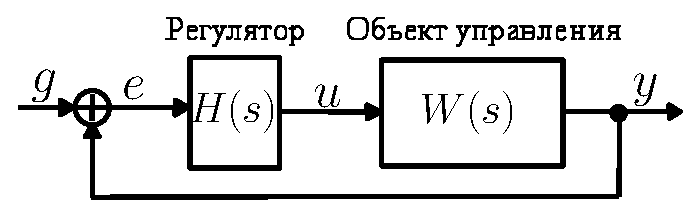
\includegraphics[width=0.6\linewidth]{cxema0.eps}
	\caption{Структурная схема моделируемой системы}
\end{figure}

\subsection{Исследование стационарного режима работы: $g(t)=A$.} 
На рисунке 2 представлена структурная схема системы при входном воздействии $g=2$, представлены графики переходных процессов (рисунок 3) и переходные характеристики ошибок (рисунок 4) при различных значениях $k$. 
\begin{figure}[h!]
	\centering
	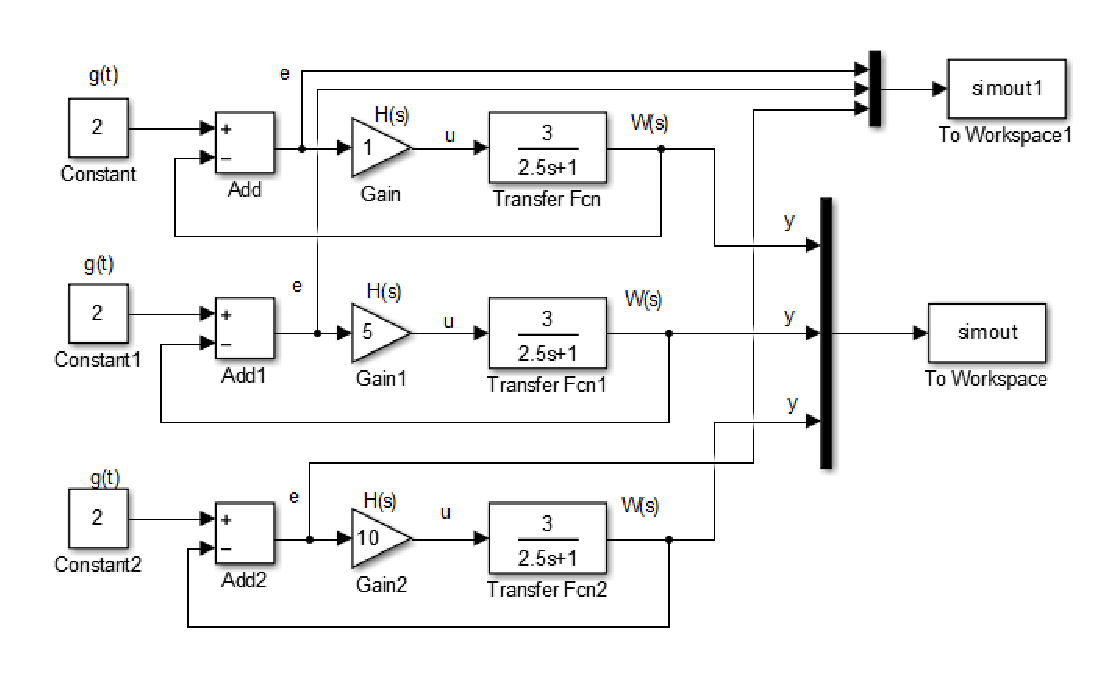
\includegraphics[width=0.8\linewidth]{cxema1.eps}
	\caption{Структурная схема системы с астатизмом нулевого порядка}
\end{figure}
\begin{figure}[H]
	\centering
	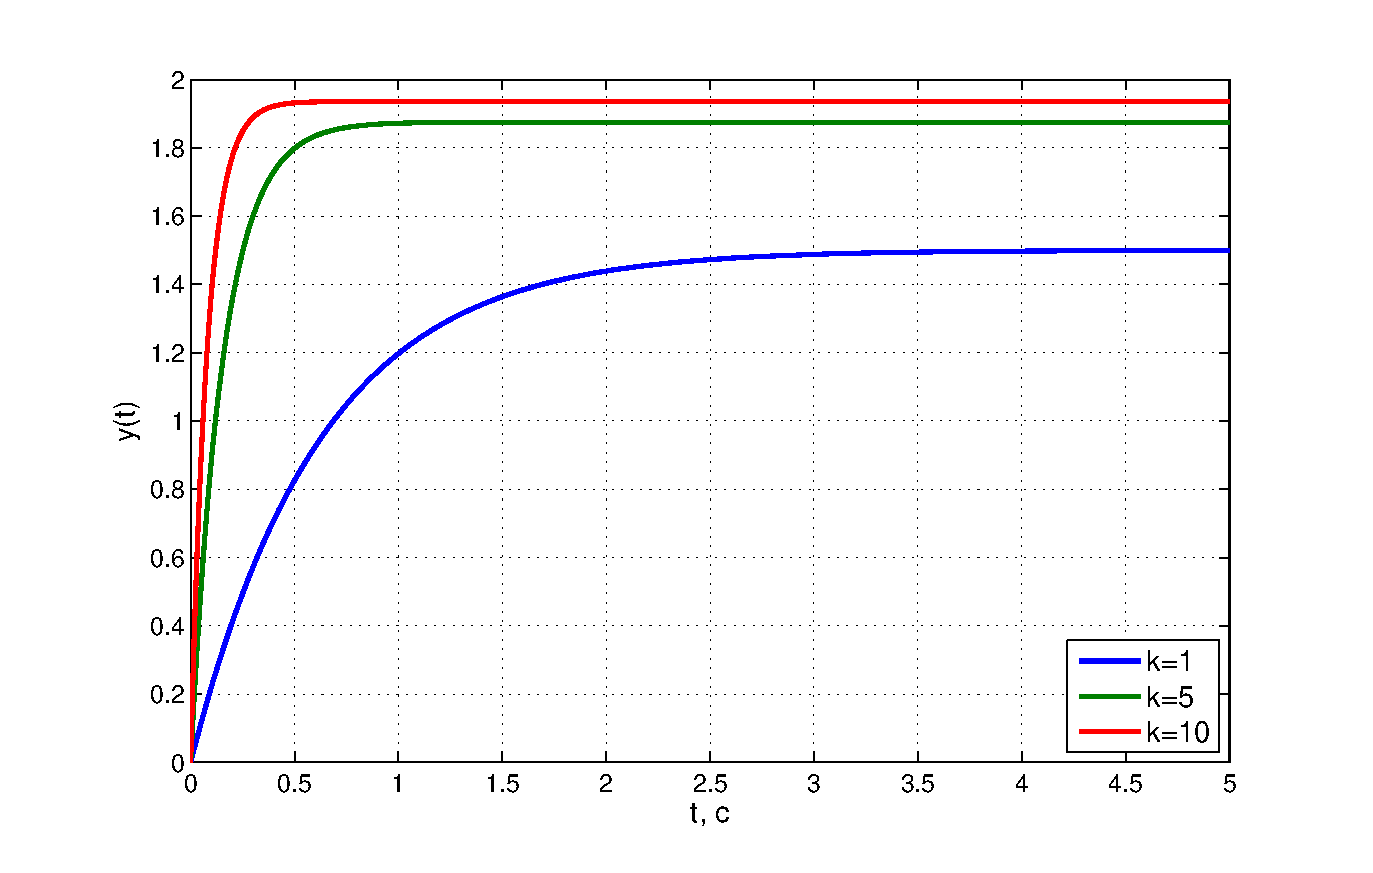
\includegraphics[width=1\linewidth]{1.1.1.eps}
	\caption{Переходные характеристики системы для стационарного режима работы}
\end{figure}
\begin{figure}[H]
	\centering
	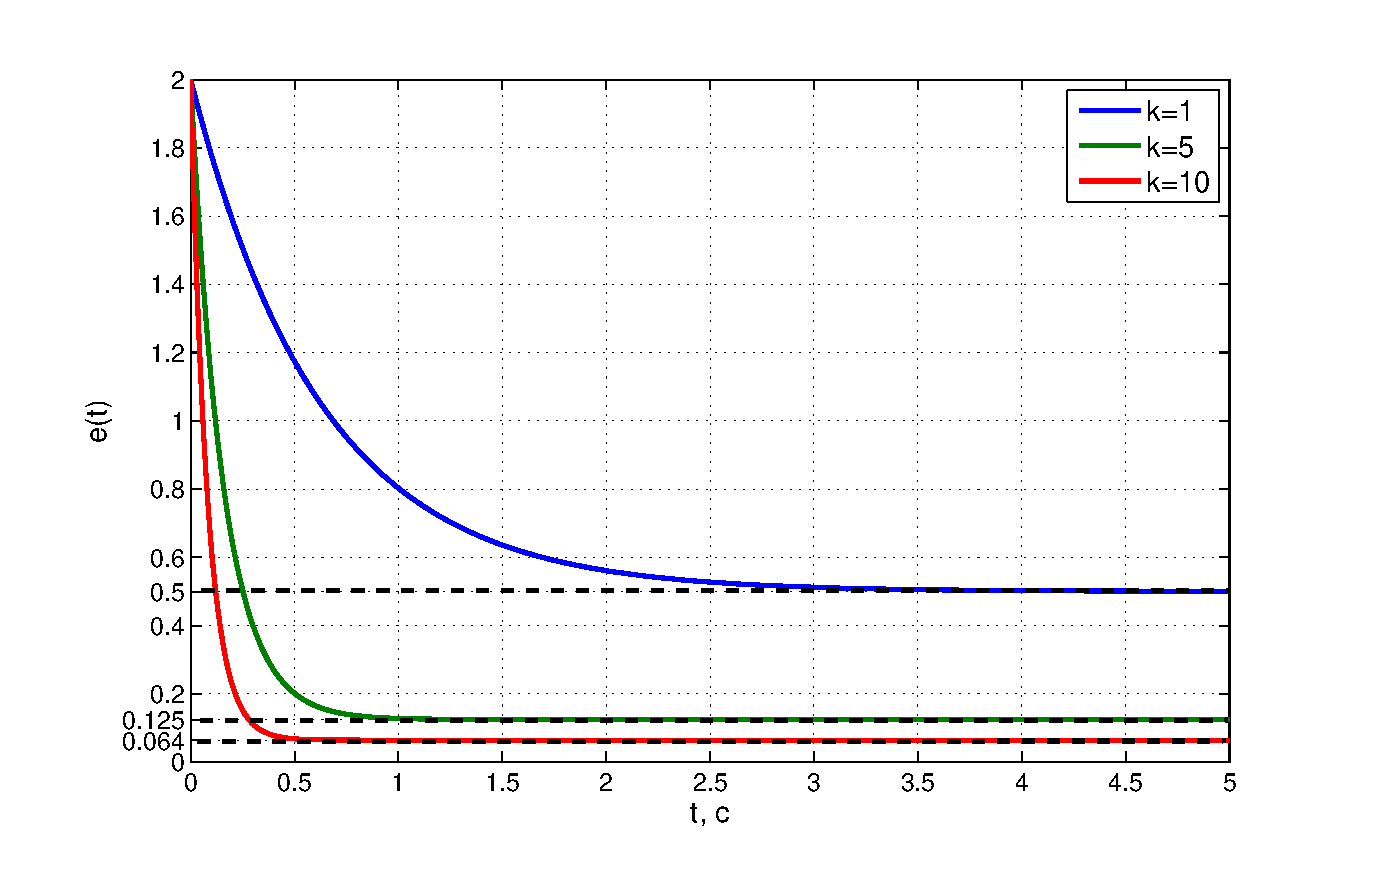
\includegraphics[width=1\linewidth]{1.1.2.eps}
	\caption{Переходные характеристики для ошибки}
\end{figure}
Для статической системы при постоянном входном воздействии $g(t)=A$ предельное значение установившейся ошибки будет равно:
\begin{equation}
    \varepsilon = \lim_{s\to 0}s\frac{1}{1+H(s)W(s)}G(s) = \lim_{s\to0} s\frac{1}{1+ \displaystyle{\frac{3k}{2,5s+1}}}\cdot\frac{A}{s} = \lim_{s\to0} \frac{5s+A}{2,5s+3k+1} = \frac{A}{1+3k}
\end{equation}
Тогда при $k=1$: $\varepsilon = \displaystyle{\frac{2}{1+1*3}} = \frac{2}{4} = 0.5;$\\
при $k=5$: $\varepsilon = \displaystyle{\frac{2}{1+5*3}} = \frac{2}{16} = 0.125;$\\
при $k=10$: $\varepsilon = \displaystyle{\frac{2}{1+10*3}} = \frac{2}{31} = 0.0645.$\\

\subsection{Исследование режима движения с постоянной скоростью: $g(t)=Vt$.} 
На рисунке 5 представлена переходная характеристика системы при входном воздействии $g=2t$.
\begin{figure}[H]
	\centering
	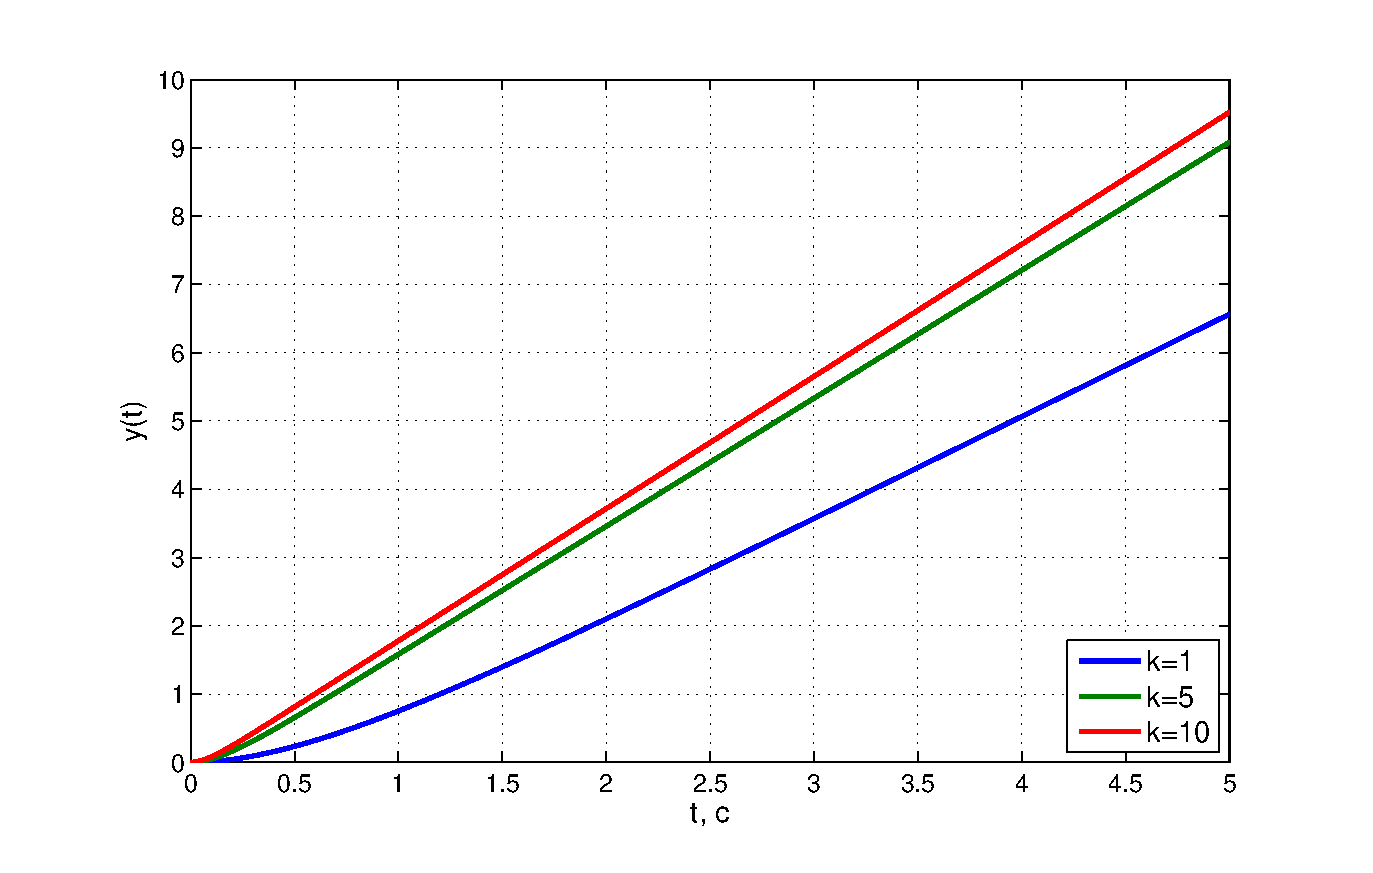
\includegraphics[width=1\linewidth]{1.2.eps}
	\caption{Переходные характеристики системы для движения с постоянной скоростью}
\end{figure}
Для статической системы при линейно нарастающем входном воздействии $g(t)=Vt$ имеем:
\begin{equation}
    \varepsilon = \lim_{s\to0} s\frac{1}{1+H(s)W(s)}G(s) = \lim_{s\to0} \frac{1}{1+\displaystyle{\frac{3k}{2.5s+1}}}\frac{V}{s} = \lim_{s\to0} \frac{V(2,5s+1)}{s(2,5s+3k+1)} = \infty
\end{equation}

\newpage
\begin{center}
\section{Исследование системы с астатизмом первого порядка}
\end{center}
Структурная схема моделируемой системы представлена на рисунке 1, где $H(s) = \displaystyle{\frac{k}{s}}, W(s)=\displaystyle{\frac{3}{2,5s + 1}}$.

\subsection{Исследование стационарного режима работы: $g(t)=A$.} 
На рисунке 6 представлена структурная схема системы при входном воздействии $g=2$, представлены графики переходных процессов (рисунок 7) и переходные характеристики ошибок (рисунок 8) при различных значениях $k$. 
\begin{figure}[H]
	\centering
	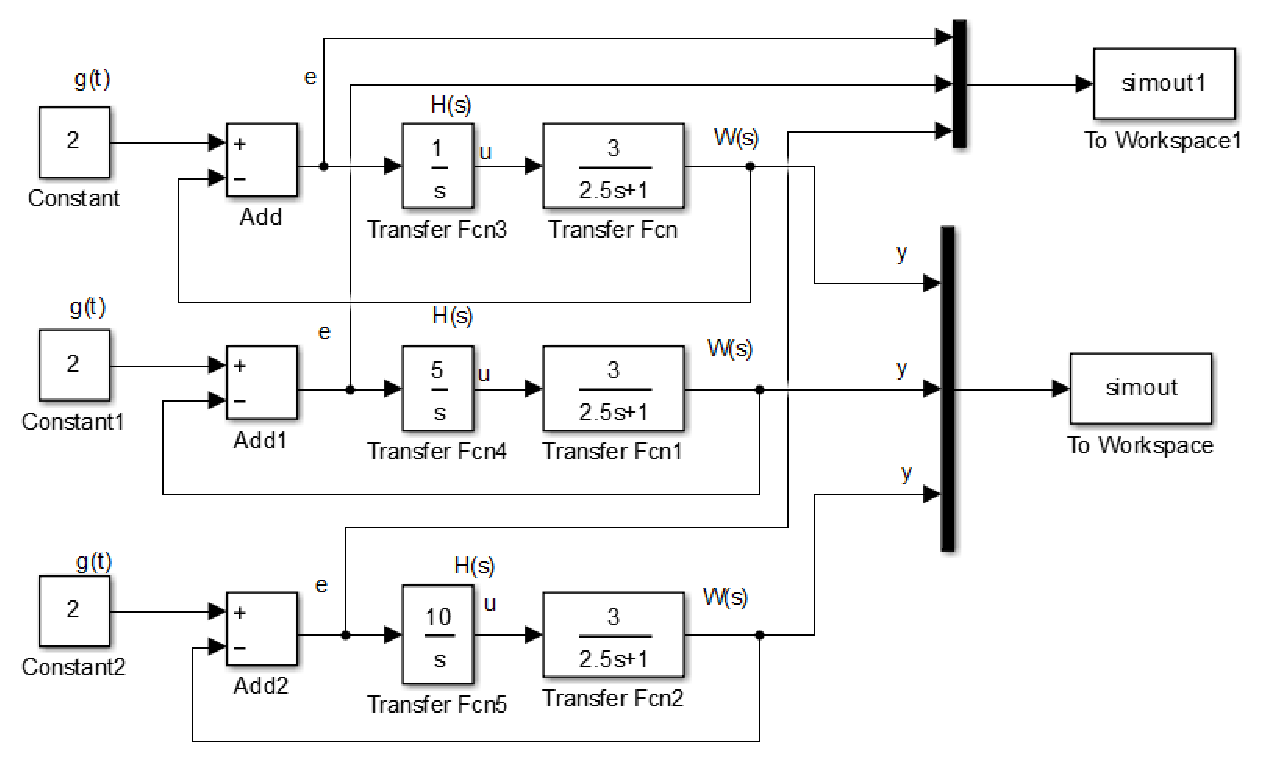
\includegraphics[width=0.8\linewidth]{cxema2.eps}
	\caption{Структурная схема системы с астатизмом нулевого порядка}
\end{figure}
Для статической системы при постоянном входном воздействии $g(t)=A$ имеем:
\begin{equation}
    \varepsilon = \lim_{s\to0} s\frac{1}{1+H(s)W(s)}G(s) = \lim_{s\to0} \frac{1}{1+\displaystyle{\frac{W^*(s)}{s}}}A = \lim_{s\to0} \frac{As(2,5s+1)}{s(2,5s+1)+3k} = \frac{0}{3k} = 0
\end{equation}
\begin{figure}[H]
	\centering
	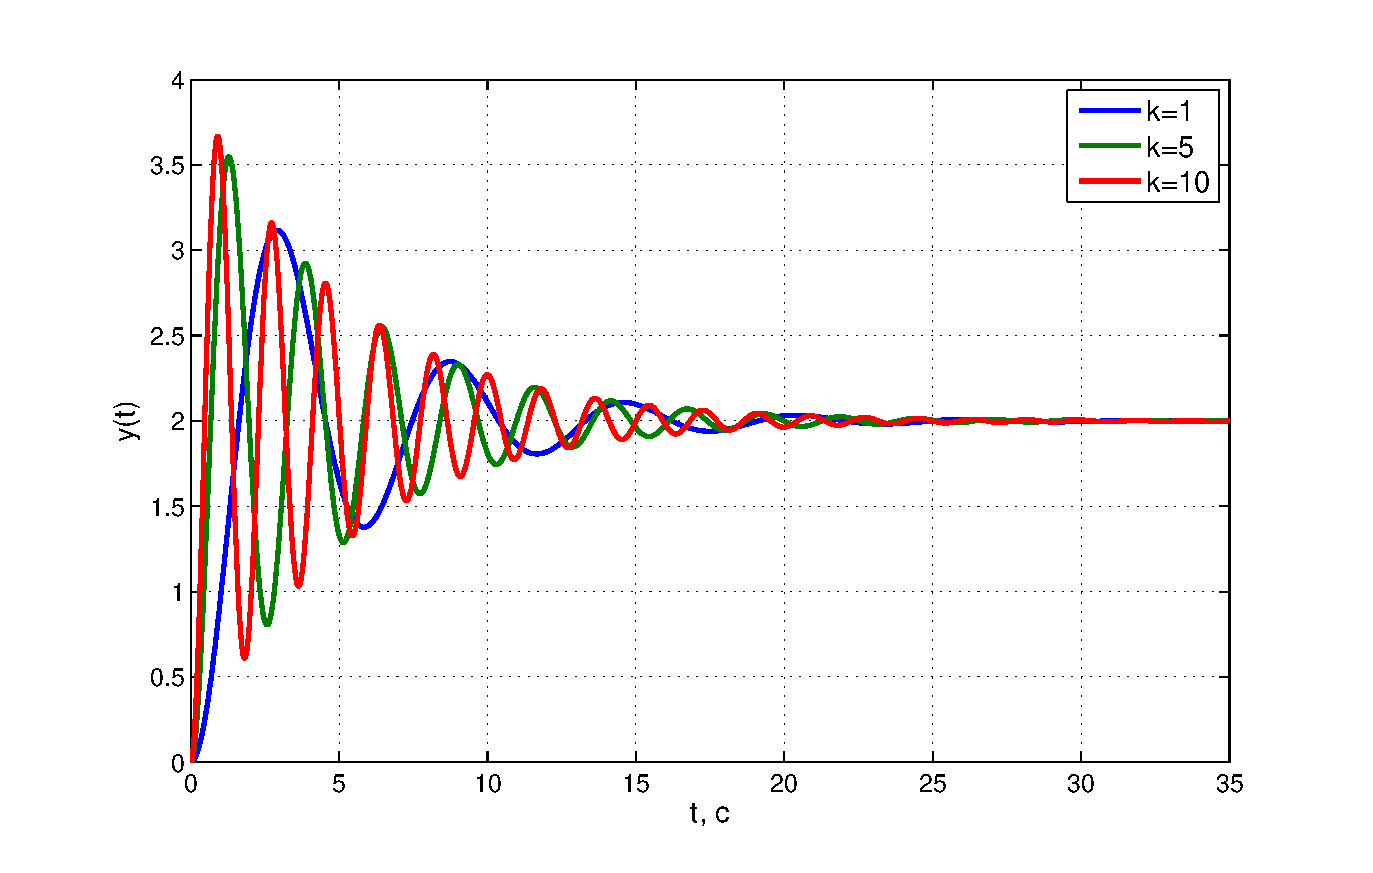
\includegraphics[width=1\linewidth]{2.1.1.eps}
	\caption{Переходные характеристики системы для стационарного режима работы}
\end{figure}
\begin{figure}[H]
	\centering
	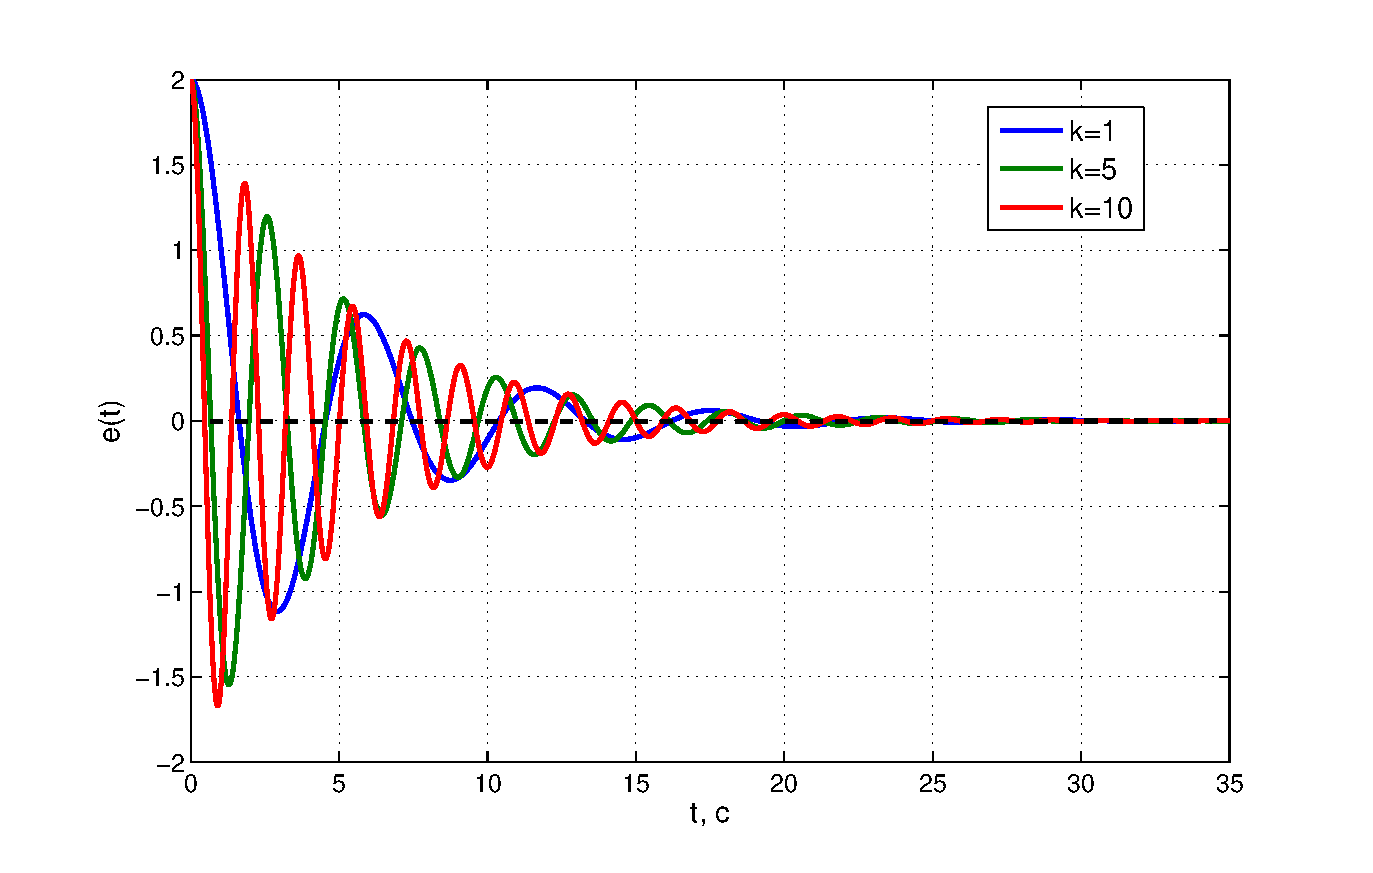
\includegraphics[width=1\linewidth]{2.1.2.eps}
	\caption{Переходные характеристики для ошибки}
\end{figure}

\subsection{Исследование режима движения с постоянной скоростью: $g(t)=Vt$.} 
На рисунке 9 представлена переходная характеристика системы при входном воздействии $g=2t$, на рисунке 10  - переходные характеристики для ошибки.
\begin{figure}[H]
	\centering
	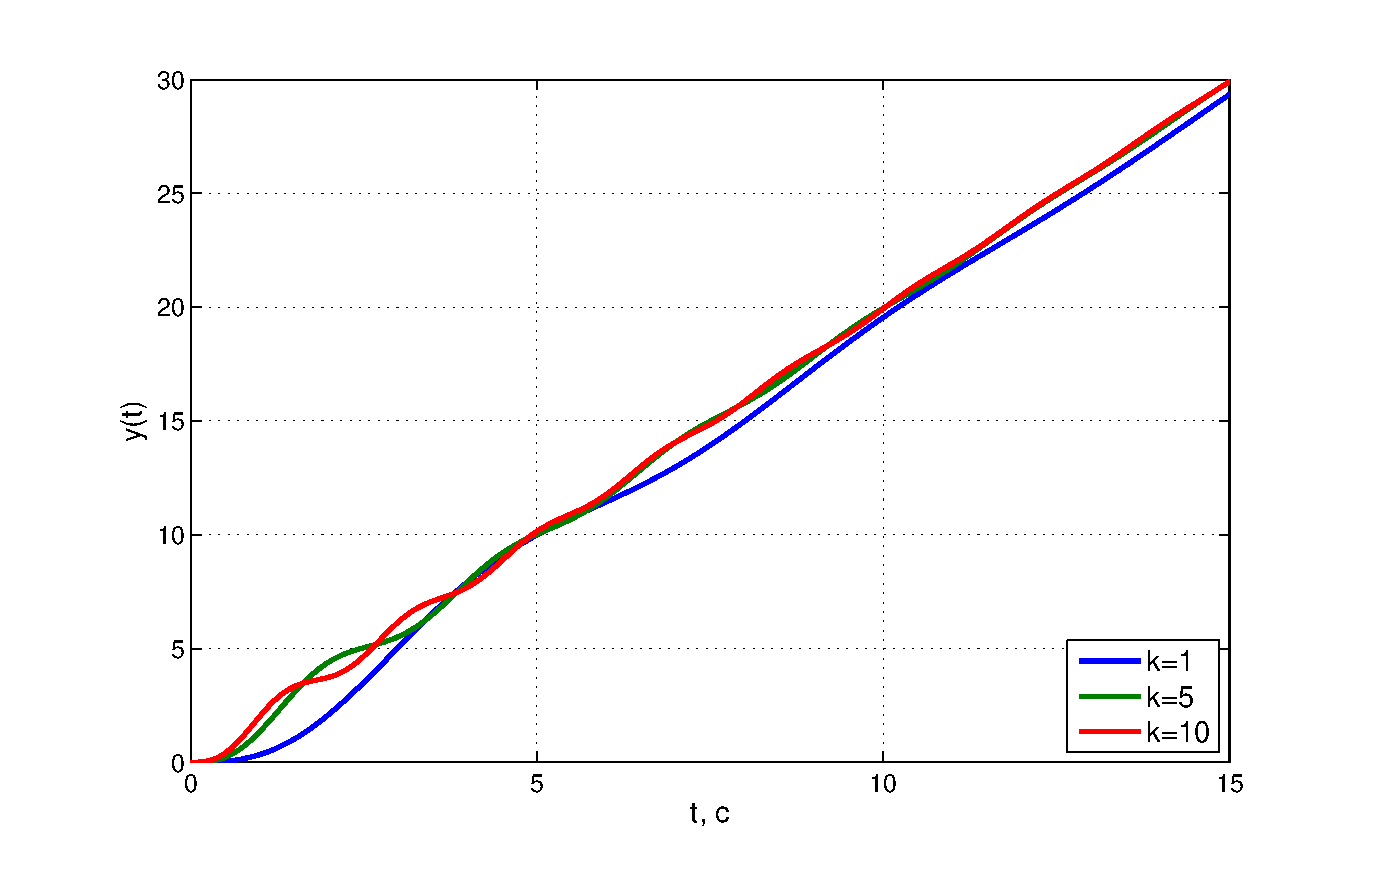
\includegraphics[width=1\linewidth]{2.2.1.eps}
	\caption{Переходные характеристики системы для движения с постоянной скоростью}
\end{figure}
При линейно нарастающем воздействии $g(t)=Vt$ предельное значение установившейся ошибки будет равно:
\begin{equation}
    \varepsilon = \lim_{s\to 0}s\frac{1}{1+H(s)W(s)}G(s) = \lim_{s\to 0}\frac{s}{1 + \displaystyle{\frac{3k}{s(2,5s+1)}}}\frac{V}{s^2} = \lim_{s\to0} \frac{V(2,5s+1)}{s(2,5s+1)+3k}= \frac{V}{3k}.
\end{equation}
Тогда при $k=1$: $\varepsilon = \displaystyle{\frac{2}{1*3} = \frac{2}{3} \approx  0.667;}$\\
при $k=5$: $\varepsilon = \displaystyle{\frac{2}{5*3} = \frac{2}{15} \approx  0.133;}$\\
при $k=10$: $\varepsilon = \displaystyle{\frac{2}{10*3} = \frac{2}{30} \approx  0.067.}$
\begin{figure}[H]
	\centering
	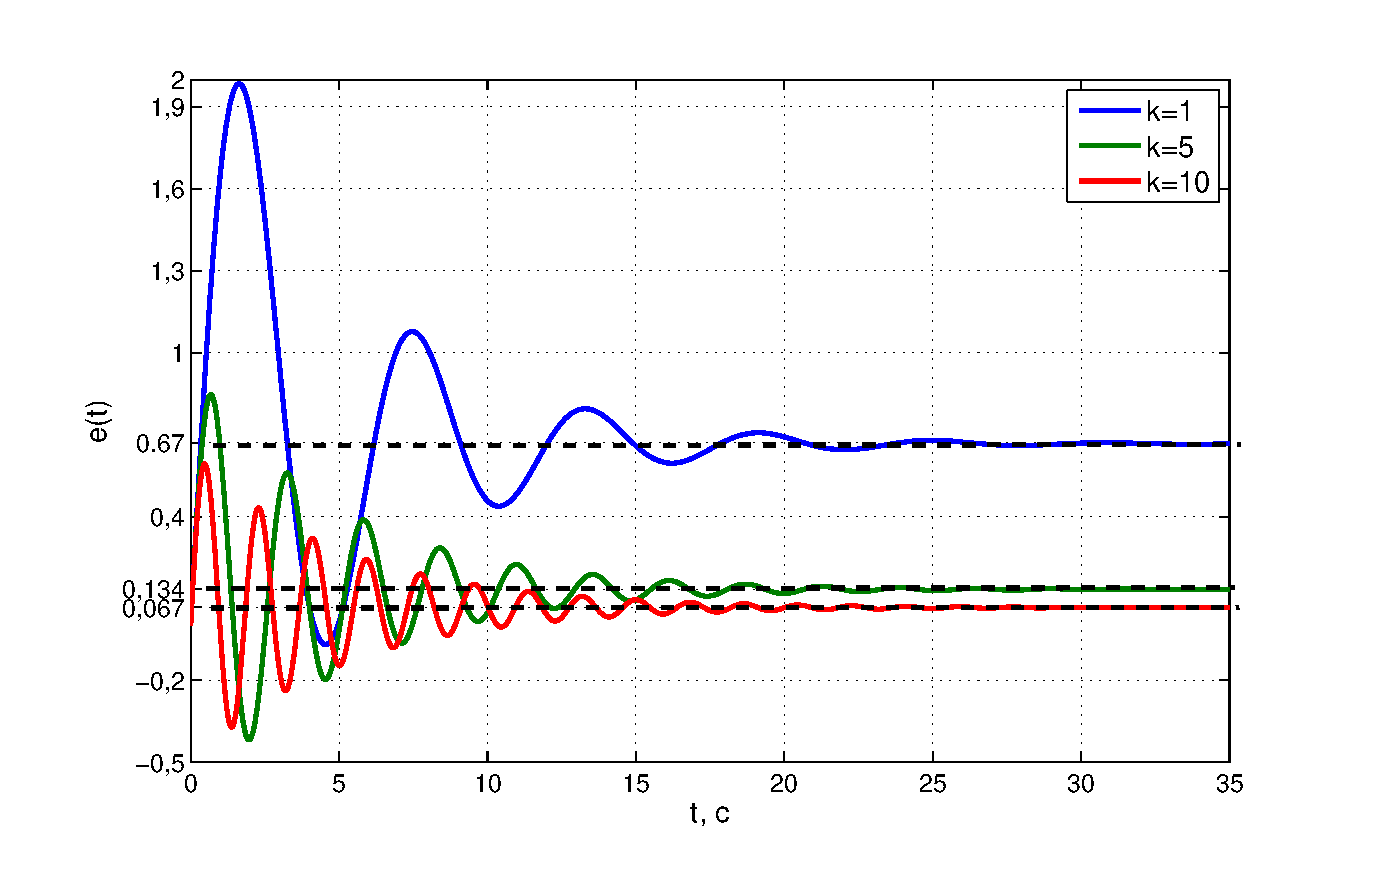
\includegraphics[width=0.95\linewidth]{2.2.2.eps}
	\caption{Переходные характеристики для ошибки}
\end{figure}

\subsection{Исследование режима движения с постоянным ускорением: $g(t)=at^2/2$.} 
На рисунке 11 представлена переходная характеристика системы при входном воздействии $g=0.5t^2$.
\begin{figure}[H]
	\centering
	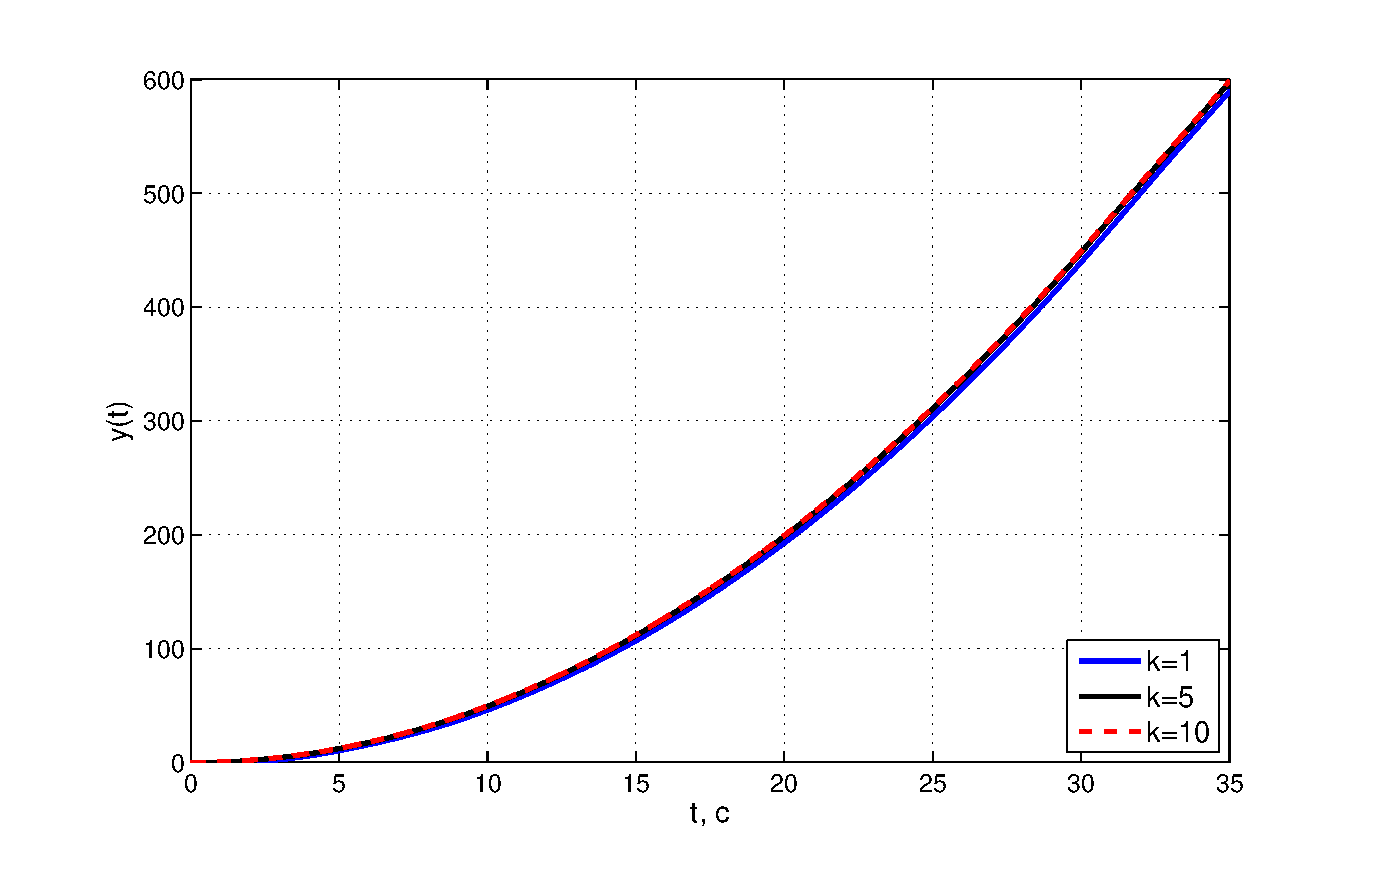
\includegraphics[width=0.95\linewidth]{2.3.eps}
	\caption{Переходные характеристики системы для движения с постоянным ускорением}
\end{figure}

\newpage
\begin{center}
\section{Исследование влияний внешних возмущений}
\end{center}
Структурная схема возмущённой системы при входном воздействии $g=1$ представлена на рисунке 12, также представлены графики переходных процессов (рисунок 13) и переходные характеристики ошибок (рисунок 14) при различных значениях $k$.
\begin{figure}[H]
    \centering
    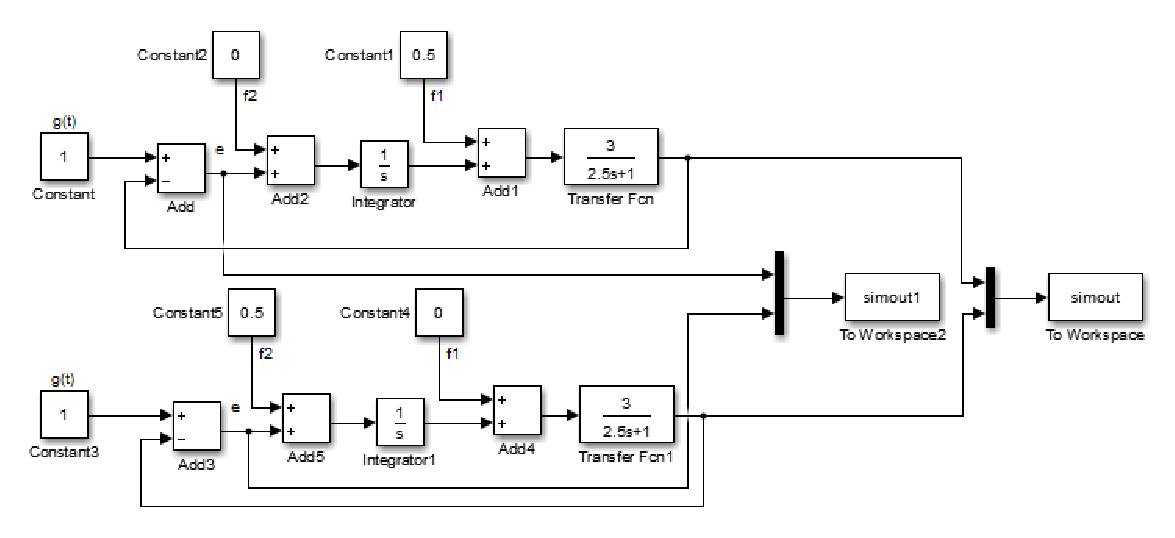
\includegraphics[width=0.8\linewidth]{cxema3.eps}
    \caption{Структурная схема системы при влиянии внешних возмущений}
\end{figure}
Функция ошибки слежения равна
\begin{equation}
e = \frac{g - W(s)f_1 - \displaystyle{\frac{1}{s}}W(s)f_2}{1 + \displaystyle{\frac{1}{s}}W(s)} = \frac{g - \displaystyle{\frac{3}{2,5s + 1}}f_1 - \displaystyle{\frac{3}{(2,5s + 1)s}}f_2}{1 + \displaystyle{\frac{3}{(2,5s + 1)s}}} = \frac{g(2,5s^2 + s) - 3sf_1 - 3f_2}{2,5s^2 + s + 3}
\end{equation}
тогда предельное значение установившейся ошибки при $g(t) = 1$
\begin{equation}
\varepsilon = \lim_{s \to 0} \frac{2,5s^2 + s - 3sf_1 - 3f_2}{2,5s^2 + s + 3} = \frac{-3f_2}{3} = -f_2.
\end{equation}
Положим, что $f_2=0$, тогда предельное значение ошибки при заданных параметрах должно быть равно 0. Если положить  $f_1=0$, тогда предельное значение ошибки будет равно $-f_2$, то есть -0.5.
\begin{figure}[H]
    \centering
    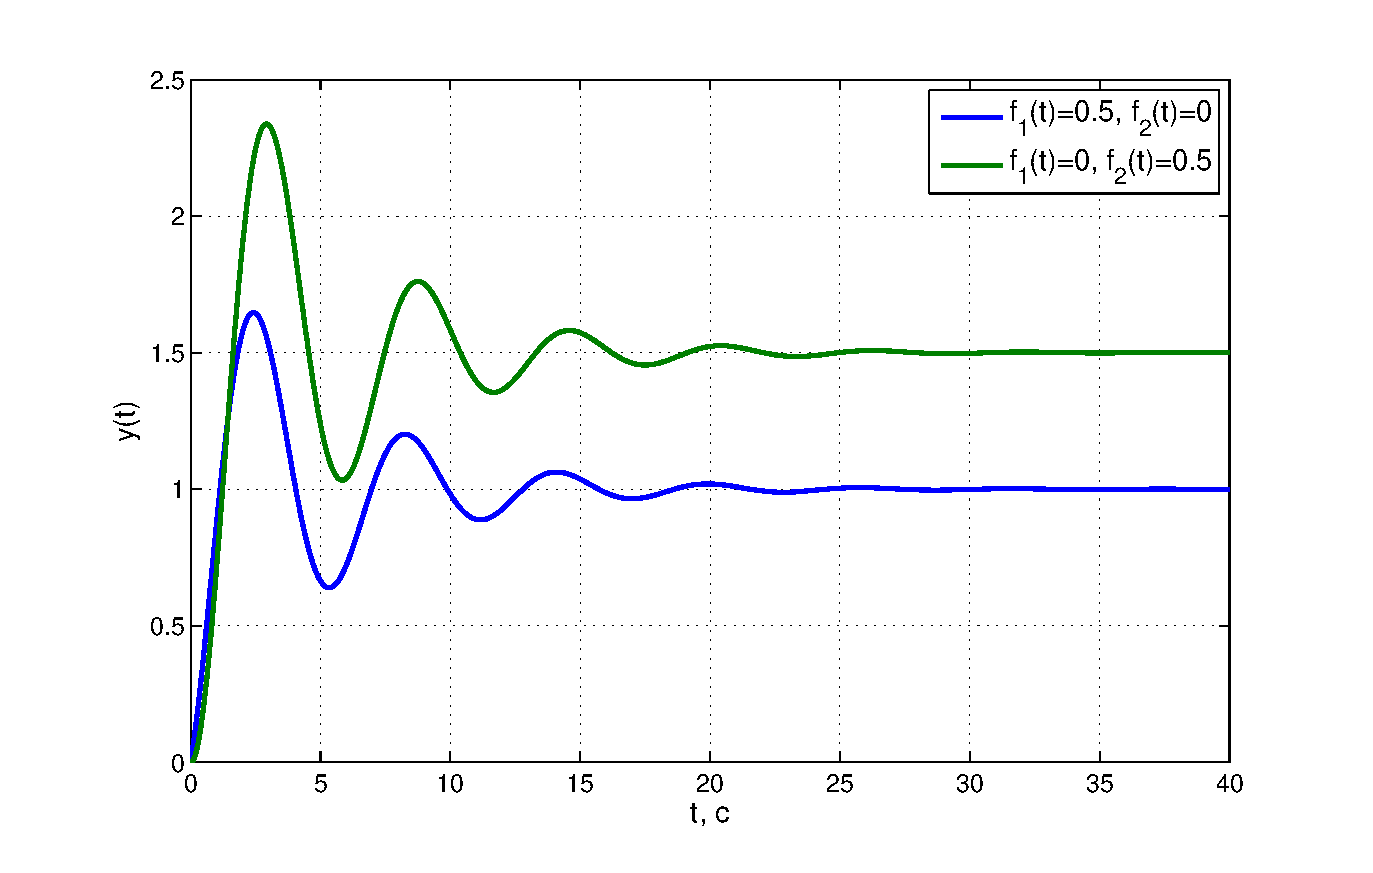
\includegraphics[width=1\linewidth]{3.1.eps}
    \caption{Переходные характеристики системы при влиянии внешних возмущений}
\end{figure}
\begin{figure}[H]
    \centering
    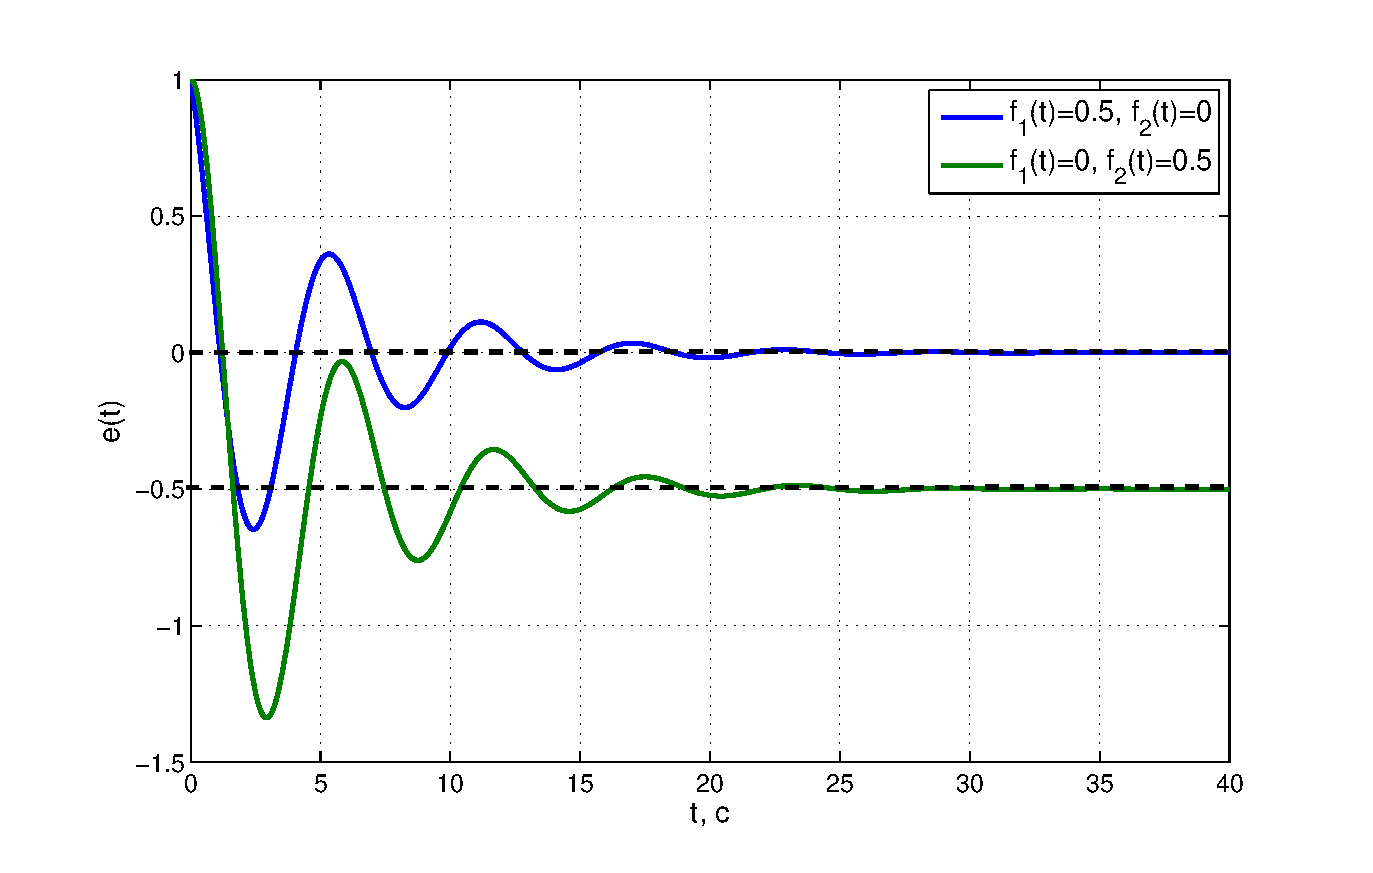
\includegraphics[width=1\linewidth]{3.2.eps}
    \caption{Переходные характеристики для ошибки}
\end{figure}

\newpage
\begin{center}
\section{Исследование установившейся ошибки при произвольном входном воздействии}
\end{center}
 Структурная схема представлена на рисунке 1, где $H(s) = 1, W(s) = \displaystyle{\frac{3}{2,5s + 1}}$, а задающее воздействие $g(t) = 0,2t^2 + \sin{0,5t}$.
 В ходе моделирования заданной системы (рисунок 15) был получен график переходного процесса, представленный на рисунке 16. Из него видно, что предельное значение ошибки стремится к $\infty$. Схема моделирования системы представленна на рисунке 13.
\begin{figure}[H]
    \centering
    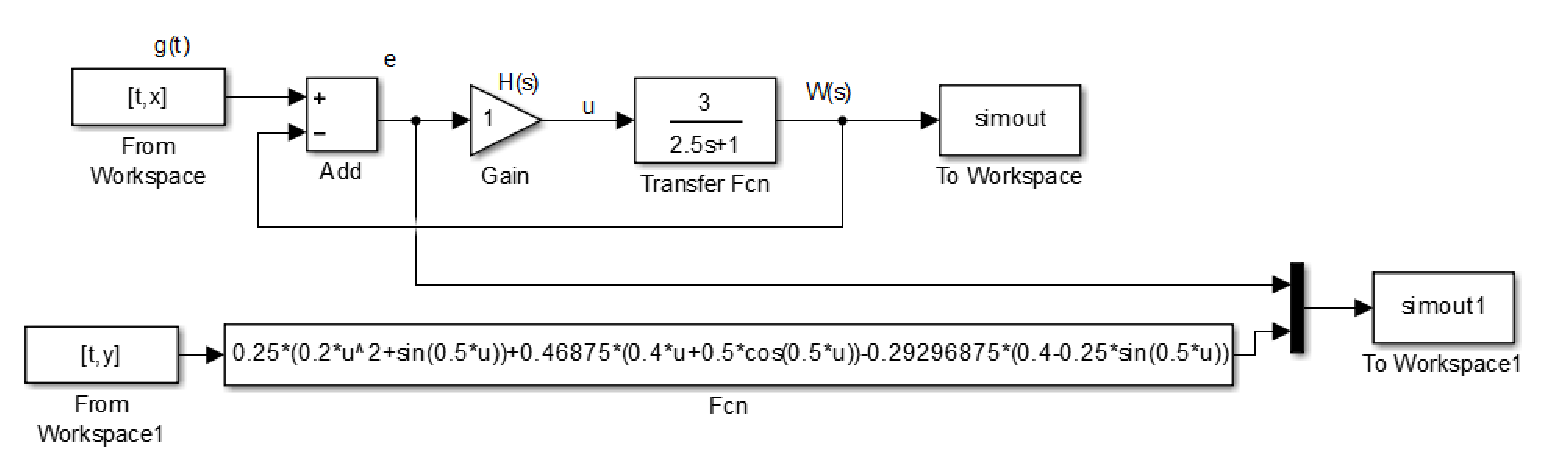
\includegraphics[width=1\linewidth]{cxema4.eps}
    \caption{Структурная схема системы при произвольном входном воздействии}
\end{figure}
\begin{figure}[H]
    \centering
    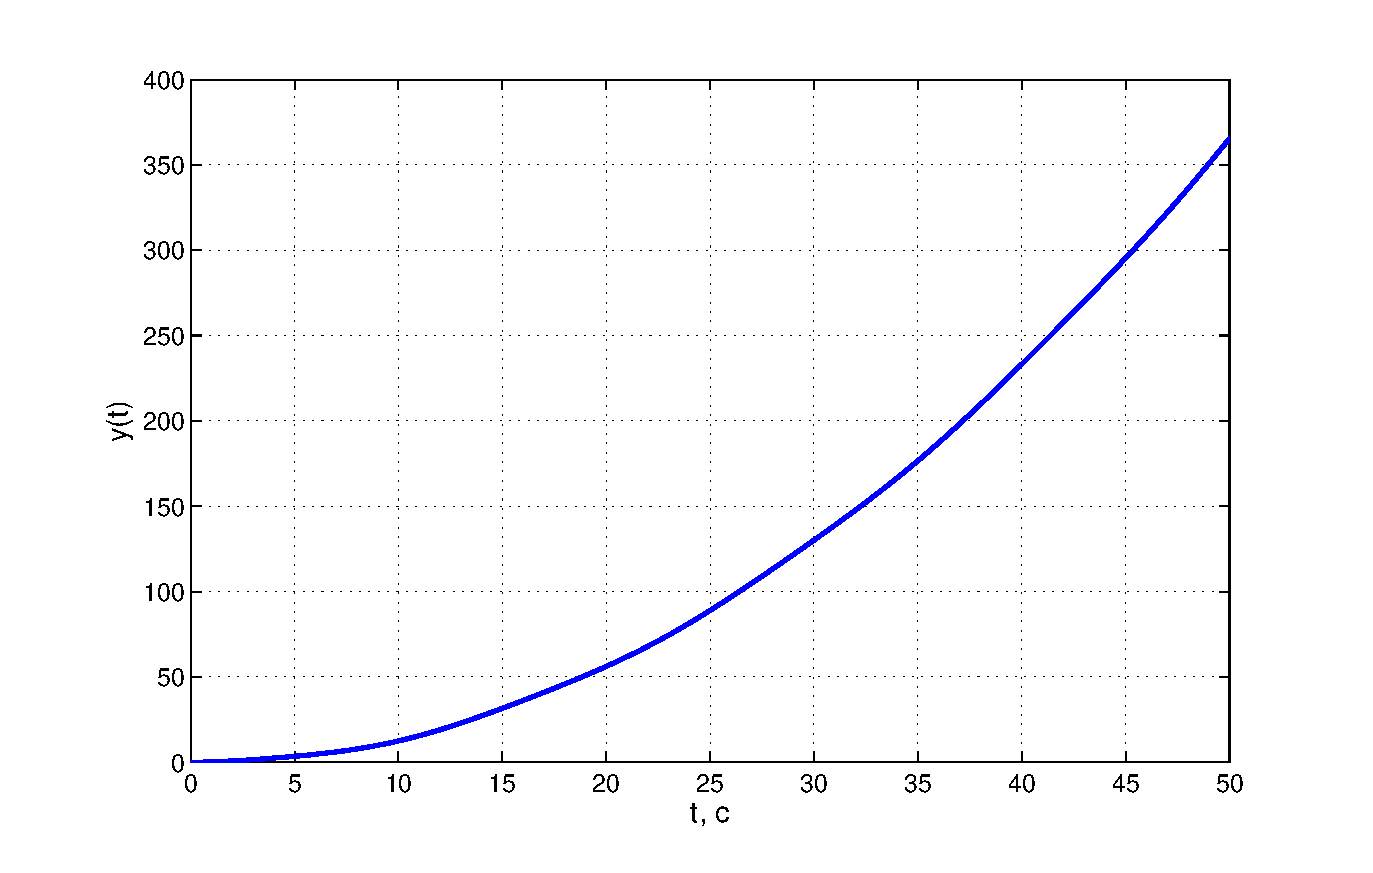
\includegraphics[width=1\linewidth]{4.1.eps}
    \caption{Переходной процесс в замкнутой системе при произвольном входном воздействии}
\end{figure}
Получим приближенное аналитическое выражение для установившейся ошибки слежения путём разложения в ряд Тейлора передаточную функцию замкнутой системы по ошибке слежения.
Передаточная функция замкнутой системы по ошибке слежения выглядит так:
\begin{equation}
   \Phi_e(s) = \frac{1}{1 + W(s)} = \frac{1}{1 + \displaystyle{\frac{3}{2,5s + 1}}} = \frac{2.5s+1}{2.5s+4}
\end{equation}\\
При произвольном входном воздействии выражение установившейся ошибки будет выглядеть следующим образом:
\begin{equation}
    e_y(t) = \Phi_e(s)|_{s=0}g(t) + \left.\frac{d\Phi_e(s)}{ds}\right|_{s=0}\dot{g}(t) + \left.\frac{d^2\Phi_e(s)}{ds^2}\right|_{s=0}\frac{\ddot{g}(t)}{2!}
\end{equation}
Найдём производные $g(t)$ и $\Phi_e(s)$:
\begin{align*}
    g(t) & = 0.2t^2 + \sin{(0.5t)} & \Phi_e(s)|_{s=0} & = \frac{2.5s+1}{2.5s+4} = 0.25 \\
    \dot{g}(t) & = 0.4t + 0.5\cos{(0.5t)} & \left.\frac{d\Phi_e(s)}{ds}\right|_{s=0} & = \frac{7.5}{(2.5s+4)^2} = 0.469 \\
    \ddot{g}(t) & = 0.4 - 0.25\sin{(0.5t)} & \left.\frac{d^2\Phi_e(s)}{ds^2}\right|_{s=0} & = \frac{-37.5}{(2.5s+4)^3} = -0.586 \\
\end{align*}
Тогда получаем выражение ошибки $e_y(t)$:
\begin{equation}
e_y(t) = 0.25(0.2t^2 + \sin{0.5t}) + 0.469(0.4t + 0.5\cos{0.5t}) - 0.293(0.4 - 0.25\sin{0.5t})
\end{equation}
Убедимся, что графики расчетной и экспериментально определённой установившейся ошибки слежения совпадают для этого построим их на одном графике, представленном на рисунке 17.
\begin{figure}[H]
    \centering
    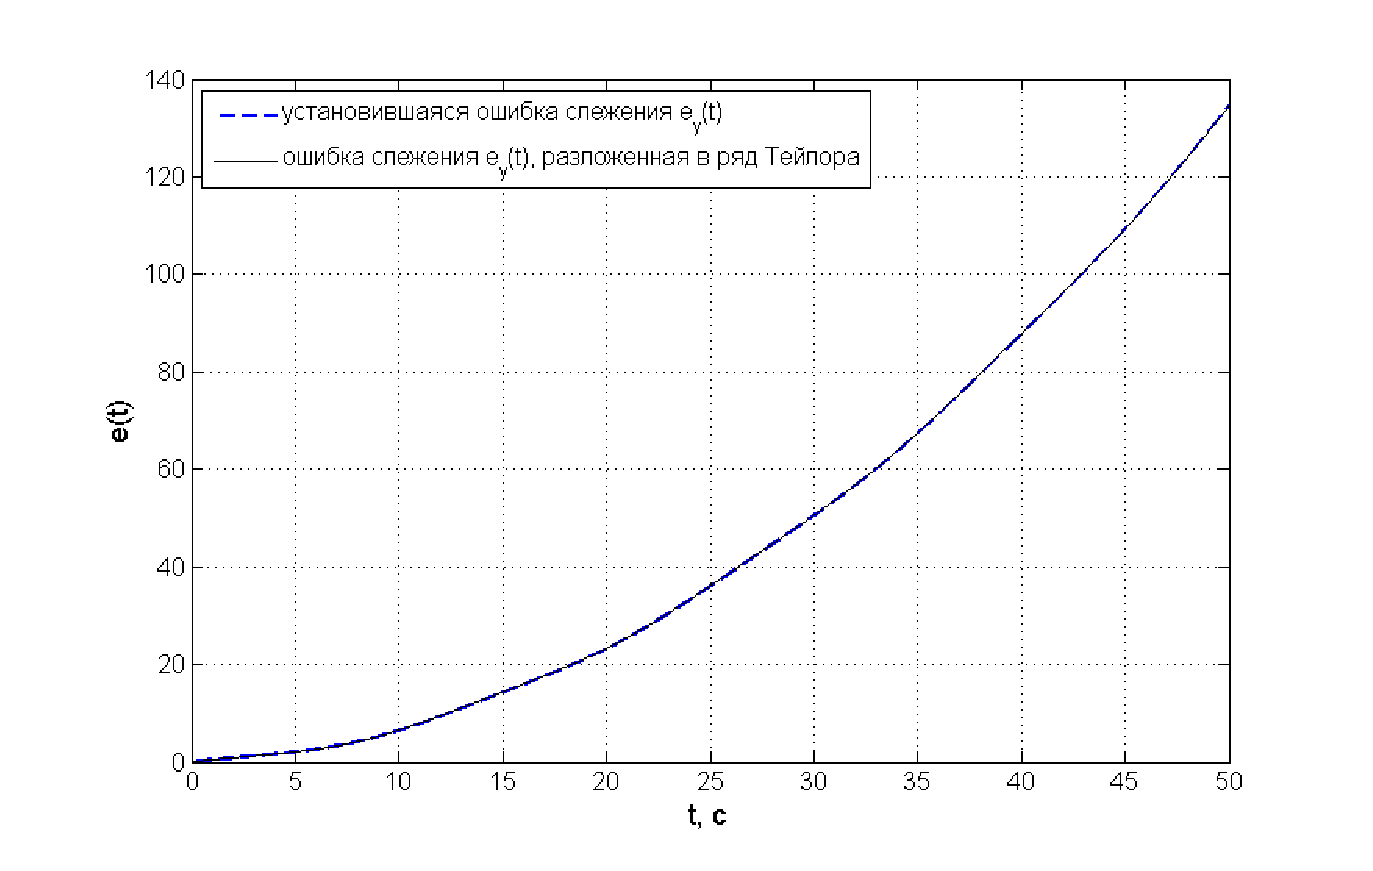
\includegraphics[width=1\linewidth]{4.2.eps}
    \caption{Графики ошибок}
\end{figure}

\newpage
\section*{Вывод}
В ходе лабораторной работы были исследованы системы с разным порядком астатизма, при влиянии внешних возмущений и при произвольном входном воздействии. Были построены переходные характеристики для всех случаев и найдены значения установившихся ошибок. Данные исследования позволяют сделать вывод о том что, установившееся значение ошибки можно изменить путём увеличения или уменьшения общего коэффициента усиления разомкнутой системы, а также путём снижения или повышения порядка астатизма.\par
Кроме того было показано, что порядок астатизма системы по задающему воздействию, в общем случае, не соответствует порядку астатизма по возмущению.\par
Так же было получено приближенное аналитическое выражение для установившейся ошибки слежения системы при произвольном входном воздействии.

\end{document}